\subsection{bpmwf/intwf.c File Reference}
\label{intwf_8c}\index{bpmwf/intwf.c@{bpmwf/intwf.c}}


\subsubsection{Detailed Description}


Definition in file {\bf intwf.c}.

{\tt \#include $<$bpm/bpm\_\-wf.h$>$}\par


Include dependency graph for intwf.c:\nopagebreak
\begin{figure}[H]
\begin{center}
\leavevmode
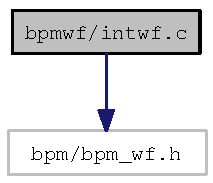
\includegraphics[width=69pt]{intwf_8c__incl}
\end{center}
\end{figure}
\subsubsection*{Functions}
\begin{CompactItemize}
\item 
{\bf intwf\_\-t} $\ast$ {\bf intwf} (int ns, double fs)
\item 
{\bf intwf\_\-t} $\ast$ {\bf intwf\_\-sample\_\-series} (int ns, double fs)
\item 
{\bf intwf\_\-t} $\ast$ {\bf intwf\_\-copy\_\-new} ({\bf intwf\_\-t} $\ast$w)
\item 
int {\bf intwf\_\-copy} ({\bf intwf\_\-t} $\ast$copy, {\bf intwf\_\-t} $\ast$src)
\item 
int {\bf intwf\_\-subset} ({\bf intwf\_\-t} $\ast$sub, {\bf intwf\_\-t} $\ast$w, int i1, int i2)
\item 
int {\bf intwf\_\-setvalues} ({\bf intwf\_\-t} $\ast$w, int $\ast$x)
\item 
int \textbf{intwf\_\-setfunction} ({\bf intwf\_\-t} $\ast$w, int($\ast$wffun)(double, int, double $\ast$), int npars, double $\ast$par)\label{intwf_8c_759d86cbc367a459aa6c593d381a2e48}

\item 
int {\bf intwf\_\-reset} ({\bf intwf\_\-t} $\ast$w)
\item 
void {\bf intwf\_\-delete} ({\bf intwf\_\-t} $\ast$w)
\item 
{\bf doublewf\_\-t} $\ast$ {\bf doublewf\_\-cast\_\-new} ({\bf intwf\_\-t} $\ast$iw)
\item 
int {\bf doublewf\_\-cast} ({\bf doublewf\_\-t} $\ast$w, {\bf intwf\_\-t} $\ast$iw)
\item 
int {\bf intwf\_\-compat} ({\bf intwf\_\-t} $\ast$w1, {\bf intwf\_\-t} $\ast$w2)
\item 
int {\bf intwf\_\-add} ({\bf intwf\_\-t} $\ast$w1, {\bf intwf\_\-t} $\ast$w2)
\item 
int {\bf intwf\_\-subtract} ({\bf intwf\_\-t} $\ast$w1, {\bf intwf\_\-t} $\ast$w2)
\item 
int {\bf intwf\_\-multiply} ({\bf intwf\_\-t} $\ast$w1, {\bf intwf\_\-t} $\ast$w2)
\item 
int {\bf intwf\_\-divide} ({\bf intwf\_\-t} $\ast$w1, {\bf intwf\_\-t} $\ast$w2)
\item 
int {\bf intwf\_\-scale} (int f, {\bf intwf\_\-t} $\ast$w)
\item 
int {\bf intwf\_\-bias} (int c, {\bf intwf\_\-t} $\ast$w)
\item 
int {\bf intwf\_\-add\_\-cwtone} ({\bf intwf\_\-t} $\ast$w, double amp, double phase, double freq, double phasenoise)
\item 
int {\bf intwf\_\-add\_\-dcywave} ({\bf intwf\_\-t} $\ast$w, double amp, double phase, double freq, double ttrig, double tdcy, double phasenoise)
\item 
int {\bf intwf\_\-add\_\-ampnoise} ({\bf intwf\_\-t} $\ast$w, double sigma)
\item 
int {\bf intwf\_\-basic\_\-stats} ({\bf intwf\_\-t} $\ast$w, int s0, int s1, {\bf wfstat\_\-t} $\ast$stats)
\item 
int {\bf intwf\_\-derive} ({\bf intwf\_\-t} $\ast$w)
\item 
int {\bf intwf\_\-integrate} ({\bf intwf\_\-t} $\ast$w)
\item 
void {\bf intwf\_\-print} (FILE $\ast$of, {\bf intwf\_\-t} $\ast$w)
\item 
int {\bf intwf\_\-getvalue} ({\bf intwf\_\-t} $\ast$w, double t, unsigned int mode)
\item 
int {\bf intwf\_\-resample} ({\bf intwf\_\-t} $\ast$w2, double fs, {\bf intwf\_\-t} $\ast$w1, unsigned int mode)
\end{CompactItemize}
